\chapter{Gaussian Process Variational Auto Encoder}\label{sec:Gaussian Process VAE}

\glspl{dvae} are a natural and straightforward extension of \glspl{vae} to the time domain. However, the discretization of time comes with limitations. First, one has to choose a relevant time interval to sample the data, which can prove arbitrary if the observed process is not well known. Second, that time interval is fixed for training and inference, can not be changed depending on the time dynamics of the observed process, and can not account for different time scales.

It is therefore interesting to allow a continuous-time formulation of the prior of the latent variables, to provide additional 
flexibility and expressiveness. A natural and straightforward framework for such a continuous time prior is the \gls{gp}, 
that constitutes the core of \glspl{gpvae}. (A summary of \gls{gp} can be found in \ref{sec:Gaussian Process}).

If the use of \glspl{gp} for time-series modeling is not recent (see for example \cite{rasmussen_gaussian_2008} and \cite{roberts_gaussian_2013}), structuring a latent prior as a \gls{gp} is somewhat newer. In \cite{casale_gaussian_2018}, Casale and al. build a \gls{gpvae} generative model to predict images with different objects and views. A specific kernel is designed for the task, taking advantage of the kernel construction rules and multiplying a view-based kernel by an object-based kernel. The kernel parameters are learnt with the inference model, and the covariance matrix of the kernel is built with a low-rank approximation ($VV^T$) to reduce computation costs (naïvely in $O(T^3)$). In \cite{fortuin_gp-vae:_2020}, Fortuin and al. focus on time-series missing values imputations. A Cauchy kernel is used, which is an instance of a Rational Quadratic Kernel, that can be viewed as an infinite sum of Gaussian kernels over the space of lengthscales. The encoder $q_\phi$ is a multivariate normal distribution, whose precision matrix is built mutliplying a bi-band matrix and its transpose, again to reduce computation cost. \cite{girin_dynamical_2022} cites \gls{gpvae} but remains focused on discrete-time models. The paper \cite{zhu_markovian_2023} establishes the Markovian nature of a \gls{gp} as the solution of a linear \gls{sde}, which allows to significantly reduce the computation cost of the model. 

The main insight is that the solution of a linear \gls{sde} is a Gaussian Process, as the transition probabilities given by the Fokker-Plank equations are Gaussian.
Thus, \glspl{gpvae} have the potential to express naturally many phenomena described by linear \glspl{sde}. 
We will review later those results, issued form stochastic calculus reference books such as \cite{mouvement-brownien-calcul-ito}, \cite{sarkka_applied_2019} and \cite{cours-jf-legall}. 

We now move to the \gls{gpvae} model itself.

We can consider \textbf{data taken at irregular time intervals}. We change our notation accordingly, and note \\
$(t_1, ..., t_{i-1}, t_i, t_{i+1}, ..., t_T)$ the $T$ times (or timestamps) considered. 

The \gls{gpm} of the \gls{gpvae} is:

\begin{figure}[H]
    \centering
    % \includegraphics[width=0.5\linewidth]{}
    \label{fig:graphical_model_gpvae}
\begin{tikzpicture}[
    HIDDEN/.style={circle, draw=black!0, thin, minimum size=10mm},
    UNOBS/.style={circle, draw=black!80, thin, minimum size=10mm},
    OBS/.style={circle, draw=black!80, fill=gray!50, thin, minimum size=10mm}
]
% nodes
\node[HIDDEN] (a) {$...$};
\node[UNOBS] (z_t_i_1) [right= of a] {$z_{t_{i-1}}$} edge[-, ultra thick] (a);
\node[UNOBS] (z_t_i)  [right= of z_t_i_1] {$z_{t_i}$} edge[-, ultra thick] (z_t_i_1);
\node[UNOBS] (z_t_i_p1) [right= of z_t_i] {$z_{t_{i+1}}$} edge[-, ultra thick] (z_t_i);
\node[HIDDEN] (e) [right= of z_t_i_p1] {$...$} edge[-, ultra thick] (z_t_i_p1);
\node[OBS] (x_t_i_1) [below= of z_t_i_1] {$x_{t_{i-1}}$} edge[<-, thin] (z_t_i_1);
\node[OBS] (x_t_i) [below= of z_t] {$x_{t_i}$} edge[<-, thin] (z_t_i);
\node[OBS] (x_t_i_p1) [below= of z_t_p1] {$x_{t_{i+1}}$} edge[<-, thin] (z_t_i_p1);
\end{tikzpicture}
\caption{Probabilistic model of a GP-VAE}
\end{figure}

Where the \textbf{thick black line} between latent variables define a fully connected graph : all latent variables are -a priori- correlated between each other in a Gaussian Process. (NB : this \gls{gpm} is not, per say, a \gls{dag} in this regard. However, D-separation still applies for observed variables $x_{t_i}$).

The joint distribution writes somehow differently from the one for \glspl{dvae}, as we put aside $p(z_{t_1:t_T})$ :
\begin{align}
\label{joint_gpvae}
    p(x_{t_1:t_T}, z_{t_1:t_T}) &= p(z_{t_1:t_T}) p(x_{t_1:t_T} \vert z_{t_1:t_T}) \\
    &= p(z_{t_1:t_T}) \prod_{i=1}^T p(x_{t_i} \vert x_{t_1:t_{i-1}}, z_{t_1:t_T}) \\
    &= p(z_{t_1:t_T}) \prod_{i=1}^T p(x_{t_i} \vert z_{t_{i}})
\end{align}

The prior over the latent variables $z_{t_i} \in \R^L$ is a set $L$ of scalar Gaussian Process over each of the dimension $l \in \{1,...,L\}$ of the latent variables. Formally:
\begin{align}
    p_{\theta_z}(z_{t_1:t_T}^l) &= \mathcal{GP}(m_{\theta_z, l}(t_1:t_T), k_{\theta_z, l}(t_1:t_T, t_1:t_T)) \hspace{1cm} l=1,..,L
\end{align}
where the $m_{\theta_z, l}$ are the $L$ mean functions of the \gls{gp} priors (usually chosen constant null), and the $k_{\theta_z, l}$ are the kernel functions of the \gls{gp} priors.

We note at this point that:
\begin{itemize}
    \item by design, each of the component prior of the $z_{t_i}$ is a scalar \gls{gp}, with correlation over time stamps. However, the different components of a $z_{t_i}$ are not correlated between them. 
    \item \textbf{The correlation across data dimensions is encoded into the observation model $p_{\theta_x}(x_{t_i} \vert z_{t_i})$}, whereas \textbf{the correlation in time is encoded into the 
    latent variable \glspl{gp}}.
    \item the kernels $k_{\theta_z, l}$ can be chosen differently to account for different prior knowledge of the data sequence. 
    In \cite{fortuin_gp-vae:_2020} for example, Fortuin and al. uses a set of Gaussian Kernels with different lenghtscales. This provides expressiveness 
    but also makes the models tricker to train.
\end{itemize}

Accordingly, the approximate posterior -encoder- $q_\phi$ is a set of $L$ Gaussian distributions of dimension $T$, each one accounting for a component of $z_{t_i}$. Formally :
\begin{align}
    q_\phi(z_{t_1:t_T}^l \vert x_{t_1:t_T}^l) &= \mathcal{N}(m_{\phi}^l(x_{t_1:t_T}), \Sigma_{\phi}^l(x_{t_1:t_T})) \hspace{1cm} l=1,..,L \\
    &= \mathcal{N}(m_{\phi}^l(x_{t_1:t_T}), \Lambda_{\phi}^l(x_{t_1:t_T})^{-1}) \\
    &= \mathcal{N}(m_{\phi}^l(x_{t_1:t_T}), L_{\phi}^l(x_{t_1:t_T})L_{\phi}^l(x_{t_1:t_T})^T)
\end{align}
where we have made explicit the different ways of defining the multivariate normal distribution, with its covariance matrix $\Sigma_\phi^l$, 
its precision matrix $\Lambda_\phi^l$, or with a Cholesky decomposition $L_{\phi}^l{L_{\phi}^l}^T$.

The observation model, by D-separation, is:
\begin{align}
\label{obs_gpvae}
    p(x_{t_1:t_T} \vert z_{t_1:t_T}) &= \prod_{i=1}^T p_{\theta_x}(x_{t_i} \vert z_{t_i})
\end{align}
The log-likelihood of the data writes:
\begin{align}
    \log{p(x_{t_1:t_T})} &= \log{\frac{p(x_{t_1:t_T}, z_{t_1:t_T})}{p(z_{t_1:t_T} \vert x_{t_1:t_T})}}
\end{align}
As usual, we multiply by $q_{\phi}(z_{t_1:t_T} \vert x_{t_1:t_T})$ and integrate over $dz_{t_1:t_T}$ to form the \gls{vlb}:
\begin{align}
    \log{p(x_{t_1:t_T})} &= \int q_{\phi}(z_{t_1:t_T} \vert x_{t_1:t_T}) \log{\frac{p(x_{t_1:t_T}, z_{t_1:t_T})}{q_{\phi}(z_{t_1:t_T}\vert x_{t_1:t_T})}\frac{q_{\phi}(z_{t_1:t_T}\vert x_{t_1:t_T})}{p(z_{t_1:t_T} \vert x_{t_1:t_T})}} dz_{t_1:t_T} \\
    &= \E{q_{\phi}(z_{t_1:t_T} \vert x_{t_1:t_T})} \log{\frac{p(x_{t_1:t_T}, z_{t_1:t_T})}{q_{\phi}(z_{t_1:t_T} \vert x_{t_1:t_T})}} + \KL{q_{\phi}(z_{t_1:t_T} \vert x_{t_1:t_T})}{p(z_{t_1:t_T} \vert x_{t_1:t_T})} \\
    &\geq \E{q_{\phi}(z_{t_1:t_T} \vert x_{t_1:t_T})} \log{\frac{p(x_{t_1:t_T}, z_{t_1:t_T})}{q_{\phi}(z_{t_1:t_T} \vert x_{t_1:t_T})}} = \VLB
\end{align}
Factoring in \ref{joint_gpvae} and \ref{obs_gpvae}, we get:
\begin{align}
    \VLB &= \E{q_{\phi}(z_{t_1:t_T} \vert x_{t_1:t_T})} \log{\left[ \left( \prod_{i=1}^T p_{\theta_x}(x_{t_i} \vert z_{t_i}) \right) \frac{p_{\theta_z}(z_{t_1:t_T})}{q_{\phi}(z_{t_1:t_T} \vert x_{t_1:t_T})}
    \right]} \\
    &= \sum_{i=1}^T \E{q_{\phi}(z_{t_1:t_T} \vert x_{t_1:t_T})} \log{p_{\theta_x}(x_{t_i} \vert z_{t_i})} - \KL{q_{\phi}(z_{t_1:t_T} \vert x_{t_1:t_T})}{p_{\theta_z}(z_{t_1:t_T})}
\end{align}
We have $\E{q_{\phi}(z_{t_1:t_T} \vert x_{t_1:t_T})} f(z_{t_i}) = \E{q_{\phi}(z_{t_i} \vert x_{t_1:t_T})} f(z_{t_i})$ for any $f$, so we get finally:
\begin{align}
    \VLB = \sum_{i=1}^T \E{q_{\phi}(z_{t_i} \vert x_{t_1:t_T})} \log{p_{\theta_x}(x_{t_i} \vert z_{t_i})} - \KL{q_{\phi}(z_{t_1:t_T} \vert x_{t_1:t_T})}{p_{\theta_z}(z_{t_1:t_T})}
\end{align}
We note that:
\begin{itemize}
    \item the $\mathbb{KL}$-divergence is actually the sum of the $L$ $\mathbb{KL}$-divergences $\KL{q_{\phi}^l}{p_{\theta_z}^l}$, which have a close form solution as both distributions are Gaussian. (see the well-known result \ref{sec:KL-two-exponential-family-distributions})
    \item the reconstruction loss term requires sampling from $q_{\phi}(z_{t_i} \vert x_{t_1:t_T})$ using the reparameterization trick as usual.
    \item the \gls{gp} priors $p_{\theta_z}(z_{t_1:t_T})$ depend only on the time stamps $t_1,...t_T$. If the kernel parameters are fixed -such as in \cite{fortuin_gp-vae:_2020}- then the priors can be computed before the training loop. If the kernel parameters are learnt with the weights of the neural nets (such as in \cite{zhu_markovian_2023}), then the computation must occur at each training iteration.
\end{itemize}

As a summary:
\begin{tcolorbox}[colback=blue!5!white,colframe=black!75!black,title=Gaussian Process VAEs]
\begin{itemize}
    \item \textbf{generative model}
    \begin{align}
        \label{gen_model_gpvae}
        p(x_{t_1:t_T}, z_{t_1:t_T}) &= p(z_{t_1:t_T}) \prod_{i=1}^T p(x_{t_i} \vert z_{t_{i}}) \\
        p_{\theta_z}(z_{t_1:t_T}^l) &= \mathcal{GP}(m_{\theta_z, l}(t_1:t_T), k_{\theta_z, l}(t_1:t_T)) \hspace{1cm} l=1,..,L
    \end{align}
    \item \textbf{inference model}
    \begin{align}
        \label{inf_model_gpvae}
        q_\phi(z_{t_1:t_T}^l \vert x_{t_1:t_T}^l) &= \mathcal{N}(m_{\phi}^l(x_{t_1:t_T}), \Sigma_{\phi}^l(x_{t_1:t_T})) \hspace{1cm} l=1,..,L \\
        &= \mathcal{N}(m_{\phi}^l(x_{t_1:t_T}), \Lambda_{\phi}^l(x_{t_1:t_T})^{-1}) \\
        &= \mathcal{N}(m_{\phi}^l(x_{t_1:t_T}), L_{\phi}^l(x_{t_1:t_T})L_{\phi}^l(x_{t_1:t_T})^T)
    \end{align}
    \item \textbf{\gls{vlb} for training}
    \begin{align}
        \label{vlb_gpvae}
        \VLB = \sum_{i=1}^T \E{q_{\phi}(z_{t_i} \vert x_{t_1:t_T})} \log{p_{\theta_x}(x_{t_i} \vert z_{t_i})} - \KL{q_{\phi}(z_{t_1:t_T} \vert x_{t_1:t_T})}{p_{\theta_z}(z_{t_1:t_T})} 
    \end{align}
\end{itemize}
\end{tcolorbox}

The PyTorch implementation is schematized here:



%
%
% ---- GP-VAE ---------------------------------
%
%

\newpage
\begin{landscape}
    
\begin{figure}
\begin{centering}
\begin{tikzpicture}[
    % format
    scale=0.55,
    every node/.style={scale=0.55},
    torch/.style={
        rectangle, 
        minimum size=6mm, 
        thick, 
        draw=green!100, 
        fill=green!20, 
        font=\ttfamily
        },
    math/.style={
        rectangle, 
        rounded corners, 
        thick, 
        draw=blue!100,
        fill=blue!20,
        align=center,
        anchor=center,
        inner sep=5pt
        },
    point/.style={
        circle,
        inner sep=0pt,
        minimum size=0pt,
        }
    ]
    % place nodes
    \matrix[row sep = 1mm, column sep=5mm] {
    % row 1
        \node[math] (xt) {
        $\begin{array}{c}
                x_{t_1:t_T} \\
                (B,T,D_x)
        \end{array}$
        }; & 
        \node[torch] (encoder) {
        $\begin{array}{c}
            \text{\ttfamily{Encoder MLP}} \\
            + \, \text{\ttfamily{torch.permute}}
        \end{array}$
        }; &
        \node[math] (zt_perm) {
        $\begin{array}{c}
                z_{t_1:t_T} \\
                (B,D_z,T)
        \end{array}$
        }; & 
        \node[math] (phi) {
            $\begin{array}{c}
                    \mu_{\phi}^l(x_{t_1:t_T}) \,\,\, (B,D_z,T)\\
                    \Sigma_{\phi}^l(x_{t_1:t_T}) \,\,\, (B,D_z,T,T) \\
                    l=1,...,D_z
            \end{array}$
        }; & 
        \node[math] (q_phi) {
        $\begin{array}{c}
        q_{\phi}^l(z_{t_1:t_T} \vert x_{t_1:t_T} ) \\
        (B,D_z) \times \mathcal{N}(T, T\times T)
        \end{array}$
        }; &
        \node[torch] (sample) {
        $\begin{array}{c}
        \text{\ttfamily{Sample}} \\
        + \, \text{\ttfamily{torch.permute}}
        \end{array}$
        }; &
        \node[math] (zt_tilde_perm) {
        $\begin{array}{c}
                \tilde{z}_{t_1:t_T} \\
                (B,T,D_z)
        \end{array}$
        }; & 
        \node[torch] (decoder) {Decoder MLP}; &
        \node[math] (theta_x) {
            $\begin{array}{c}
                    \mu_{\theta_x}^t(z_{t_1:t_T}) \,\,\, (B,T,D_x)\\
                    \Sigma_{\theta_x}^t(z_{t_1:t_T}) \,\,\, (B,T,D_x,D_x) \\
                    t=1,...,T
            \end{array}$
        }; & 
        \node[math] (p_theta_x) {
        $\begin{array}{c}
        p_{\theta_x}(x_{t_1:t_T} \vert \tilde{z}_{t_1:t_T} ) \\ 
        (B,T) \times \mathcal{N}(D_x, D_x\times D_x) \\
        \end{array}$
        }; & \\
    % row 2
    \node[math] (times) {
        $\begin{array}{c}
                {t_1:t_T} \\
                (B,T,1)
        \end{array}$
        }; & &  
    \node[torch] (prior) {GP Prior}; &
    \node[math] (theta_z) {
            $\begin{array}{c}
                    m_{\theta_z, l}({t_1:t_T}) \,\,\, (B,D_z,T)\\
                    k_{\theta_z, l}({t_1:t_T,t_1:t_T}) \,\,\, (B,D_z,T,T) \\
                    l=1,...,D_z
            \end{array}$
        }; &  
    \node[math] (p_theta_z) {
        $\begin{array}{c}
        p_{\theta_z}({t_1:t_T}) \\ 
        (B,D_z) \times \mathcal{N}(T, T\times T) \\
        \end{array}$
        }; & \\
    };
    % draw edges
    \path   (xt) edge [->, thin] (encoder)
            (encoder) edge [->, thin] (zt_perm)
            (zt_perm) edge [->, thin] (phi)
            (phi) edge [->, thin] (q_phi)
            (q_phi) edge [->, thin] (sample)
            (sample) edge [->, thin] (zt_tilde_perm)
            (zt_tilde_perm) edge [->, thin] (decoder)
            (decoder) edge [->, thin] (theta_x)
            (theta_x) edge [->, thin] (p_theta_x)
            (times) edge[->, thin] (prior)
            (prior) edge[->, thin] (theta_z)
            (theta_z) edge[->, thin] (p_theta_z);
\end{tikzpicture}

% --- Loss GPVAE
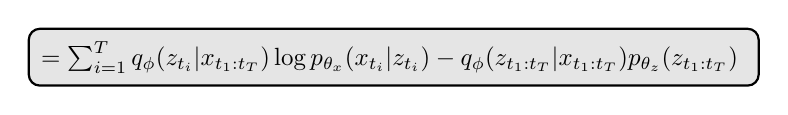
\begin{tikzpicture}[
    scale=0.90,
    every node/.style={scale=0.90},
    math/.style={
        rectangle, 
        % minimum height=1cm,
        % minimum width=2cm,
        rounded corners, 
        thick, 
        draw=black!100,
        fill=gray!20,
        align=center,
        anchor=center,
        inner sep=5pt
        },
    ]
    \node[math] {
        $\VLB = \sum_{i=1}^T \E{q_{\phi}(z_{t_i} \vert x_{t_1:t_T})} \log{p_{\theta_x}(x_{t_i} \vert z_{t_i})} - \KL{q_{\phi}(z_{t_1:t_T} \vert x_{t_1:t_T})}{p_{\theta_z}(z_{t_1:t_T})}$
    };
\end{tikzpicture}

\caption{Gaussian Process VAE Model Architecture}
\end{centering}
\end{figure}

\end{landscape}

         